\documentclass{beamer}

\usefonttheme{professionalfonts} % using non standard fonts for beamer
\usefonttheme{serif} % default family is serif

\usepackage{hyperref}
%\usepackage{minted}
\usepackage{animate}
\usepackage{graphicx}
\def\Put(#1,#2)#3{\leavevmode\makebox(0,0){\put(#1,#2){#3}}}
\usepackage{colortbl}
\usepackage{tikz}
\usepackage{amssymb}
\usepackage{enumerate}
\usepackage{arydshln}
\usepackage{algorithm}
\usepackage{algpseudocode}

\colorlet{lightred}{red!25}
\colorlet{lightgreen}{green!25}


\newcommand\blfootnote[1]{%

  \begingroup

  \renewcommand\thefootnote{}\footnote{#1}%

  \addtocounter{footnote}{-1}%

  \endgroup

}

\makeatletter

%%%%%%%%%%%%%%%%%%%%%%%%%%%%%% Textclass specific LaTeX commands.

 % this default might be overridden by plain title style

 \newcommand\makebeamertitle{\frame{\maketitle}}%

 % (ERT) argument for the TOC

 \AtBeginDocument{%

   \let\origtableofcontents=\tableofcontents

   \def\tableofcontents{\@ifnextchar[{\origtableofcontents}{\gobbletableofcontents}}

   \def\gobbletableofcontents#1{\origtableofcontents}

 }

%%%%%%%%%%%%%%%%%%%%%%%%%%%%%% User specified LaTeX commands.

\usetheme{Malmoe}

% or ...

\useoutertheme{infolines}

\addtobeamertemplate{headline}{}{\vskip2pt}

\setbeamercovered{transparent}

% or whatever (possibly just delete it)

\makeatother

\begin{document}
\title[PFLOCK report]{PFLOCK Report}
\author[AC]{Andres Calderon}
\institute[Spring'20]{University of California, Riverside}
\makebeamertitle
\newif\iflattersubsect

\AtBeginSection[] {
    \begin{frame}<beamer>
    \frametitle{Outline} 
    \tableofcontents[currentsection]  
    \end{frame}
    \lattersubsectfalse
}

\AtBeginSubsection[] {
    \begin{frame}<beamer>
    \frametitle{Outline} 
    \tableofcontents[currentsubsection]  
    \end{frame}
}

\begin{frame}{Points...}
    \centering
    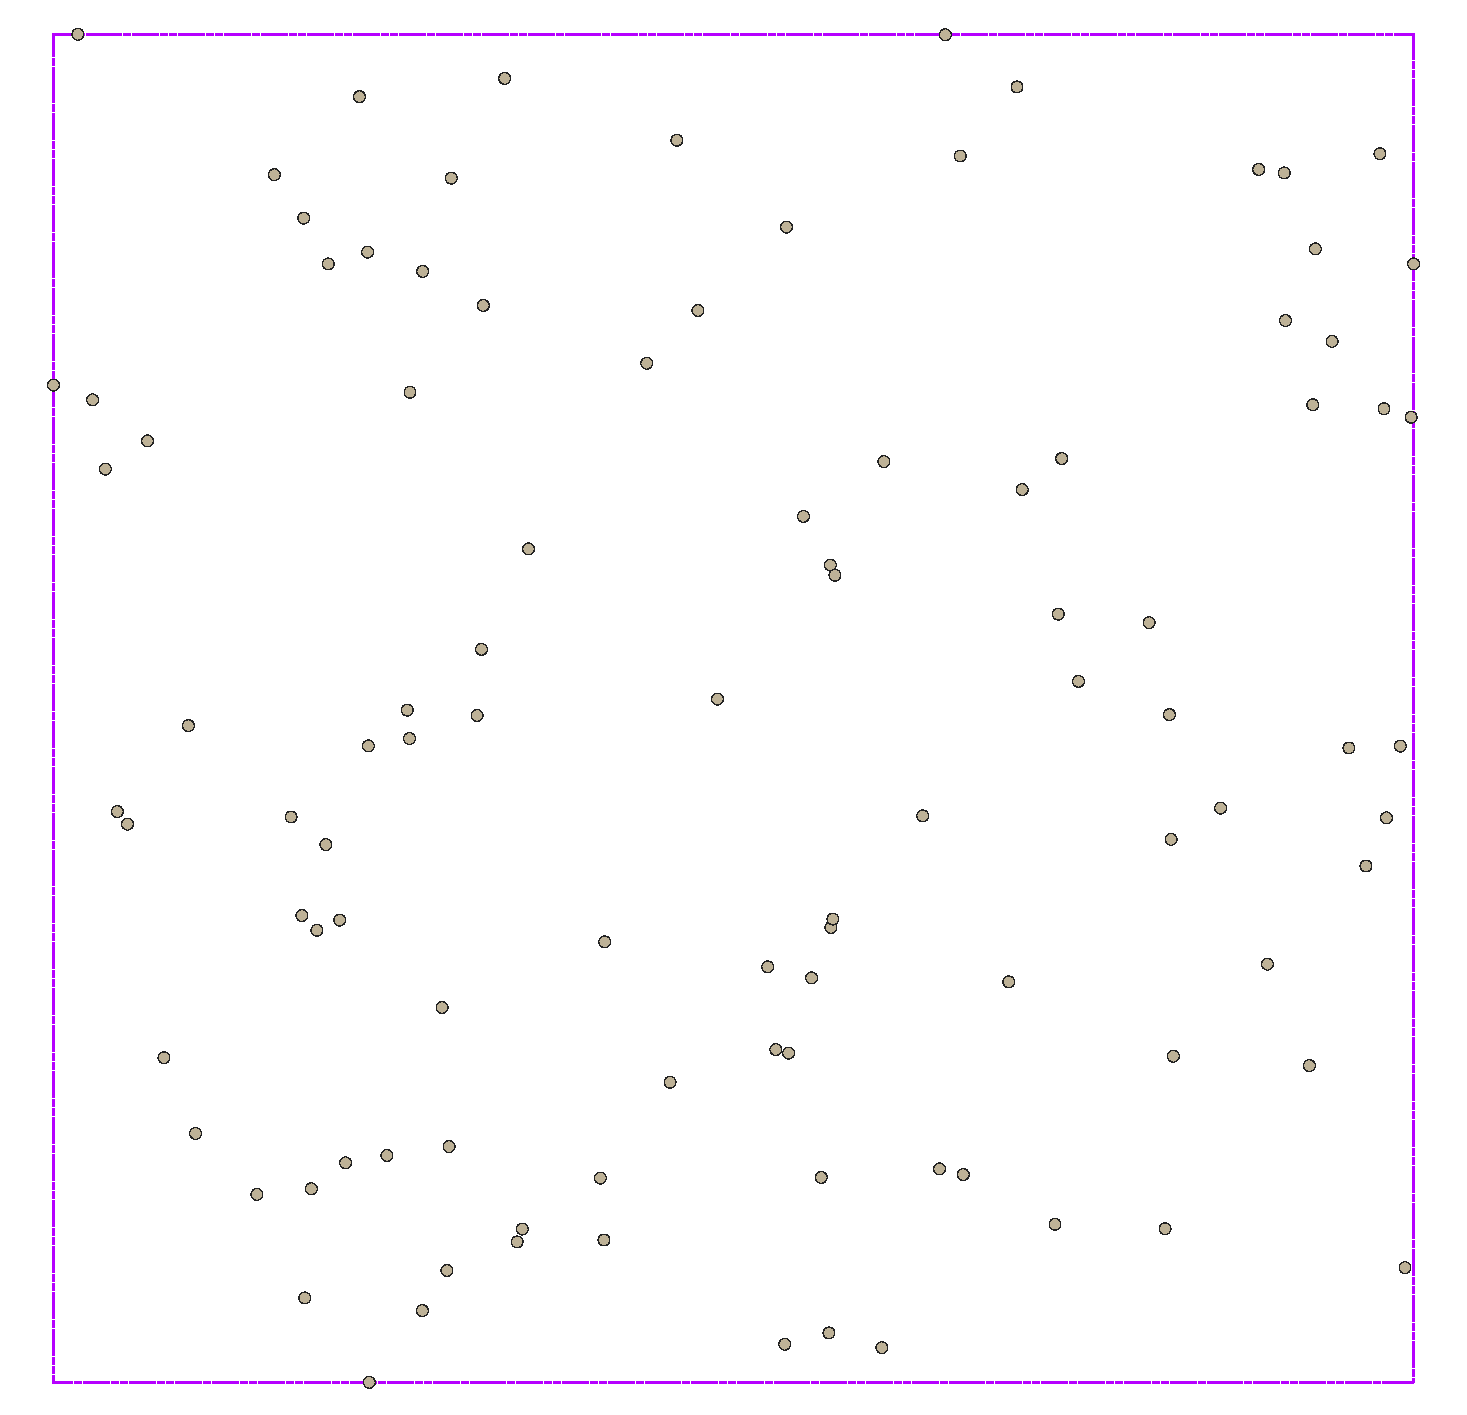
\includegraphics[width=0.65\textwidth]{figures/01-Points}
\end{frame}
\begin{frame}{Global Partitions...}
    \centering
    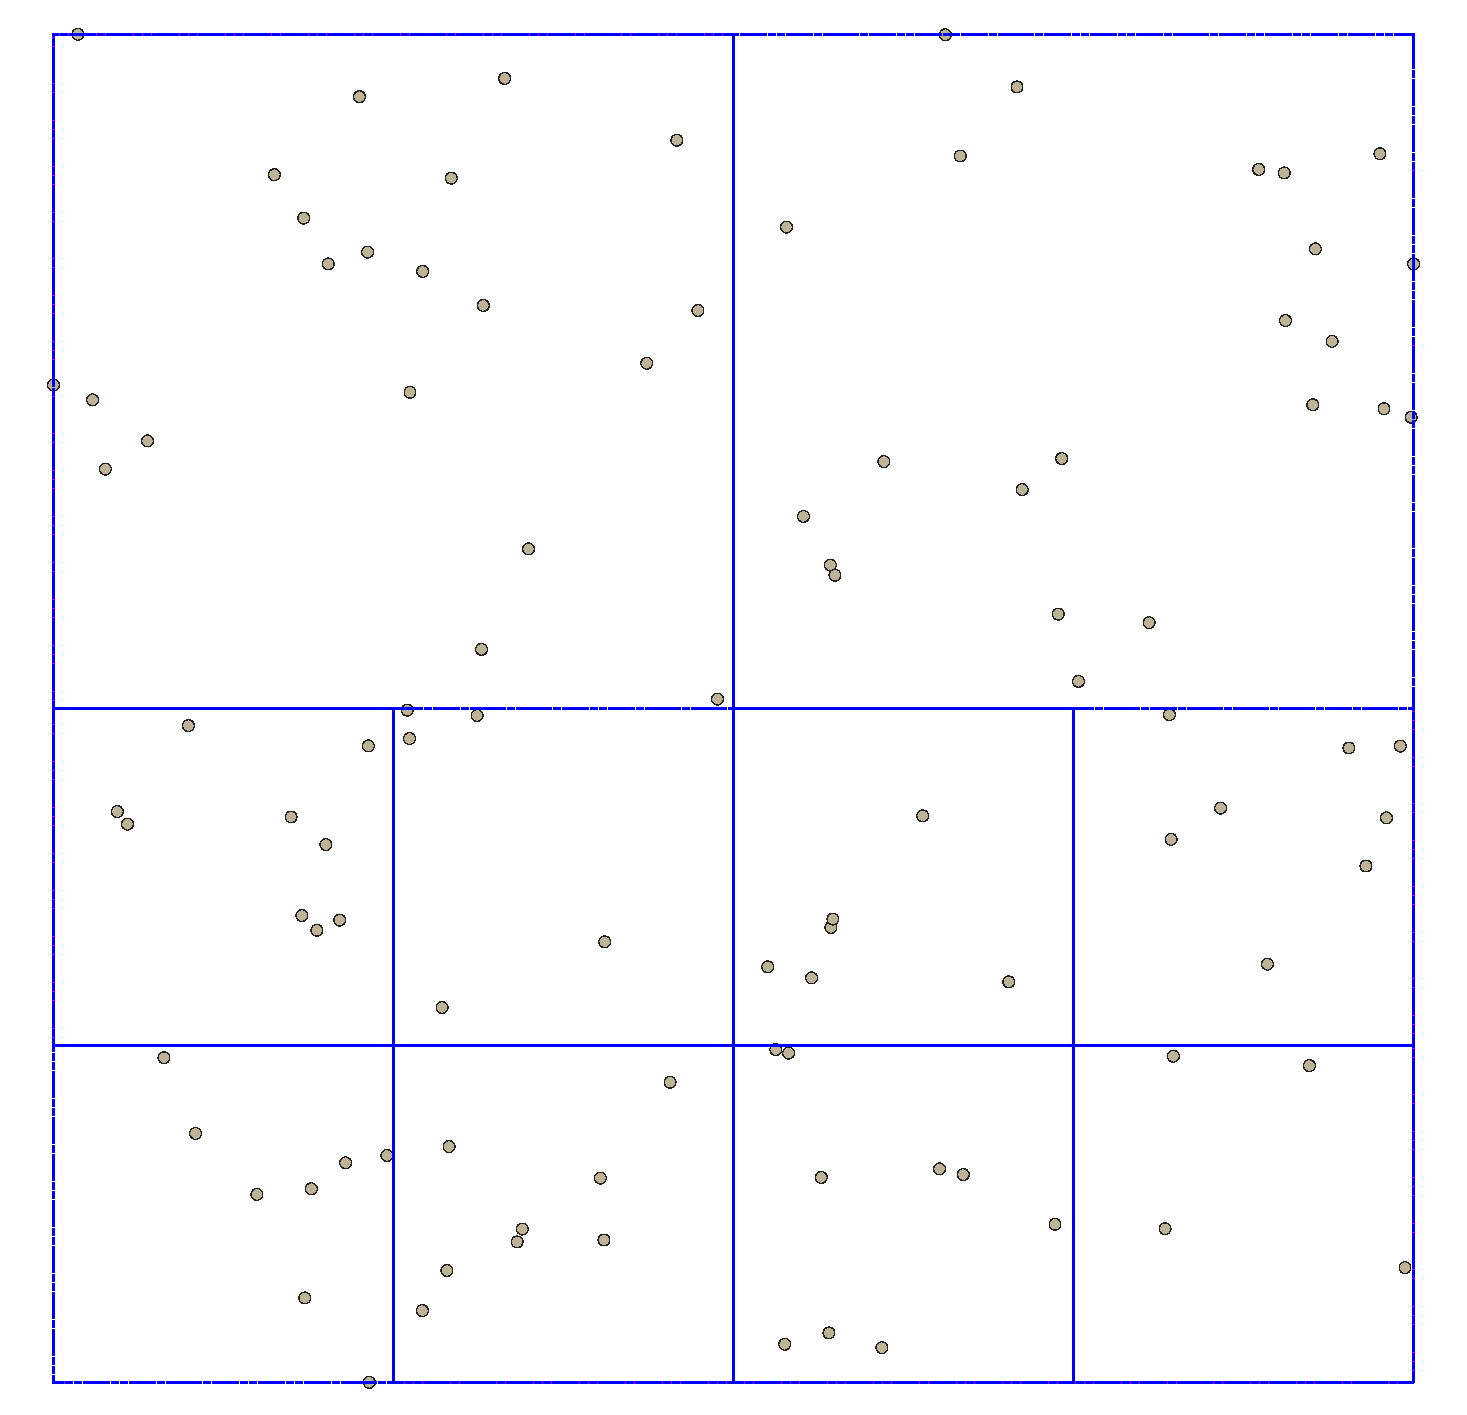
\includegraphics[width=0.65\textwidth]{figures/02-GPartitions}
\end{frame}
\begin{frame}{Centers...}
    \centering
    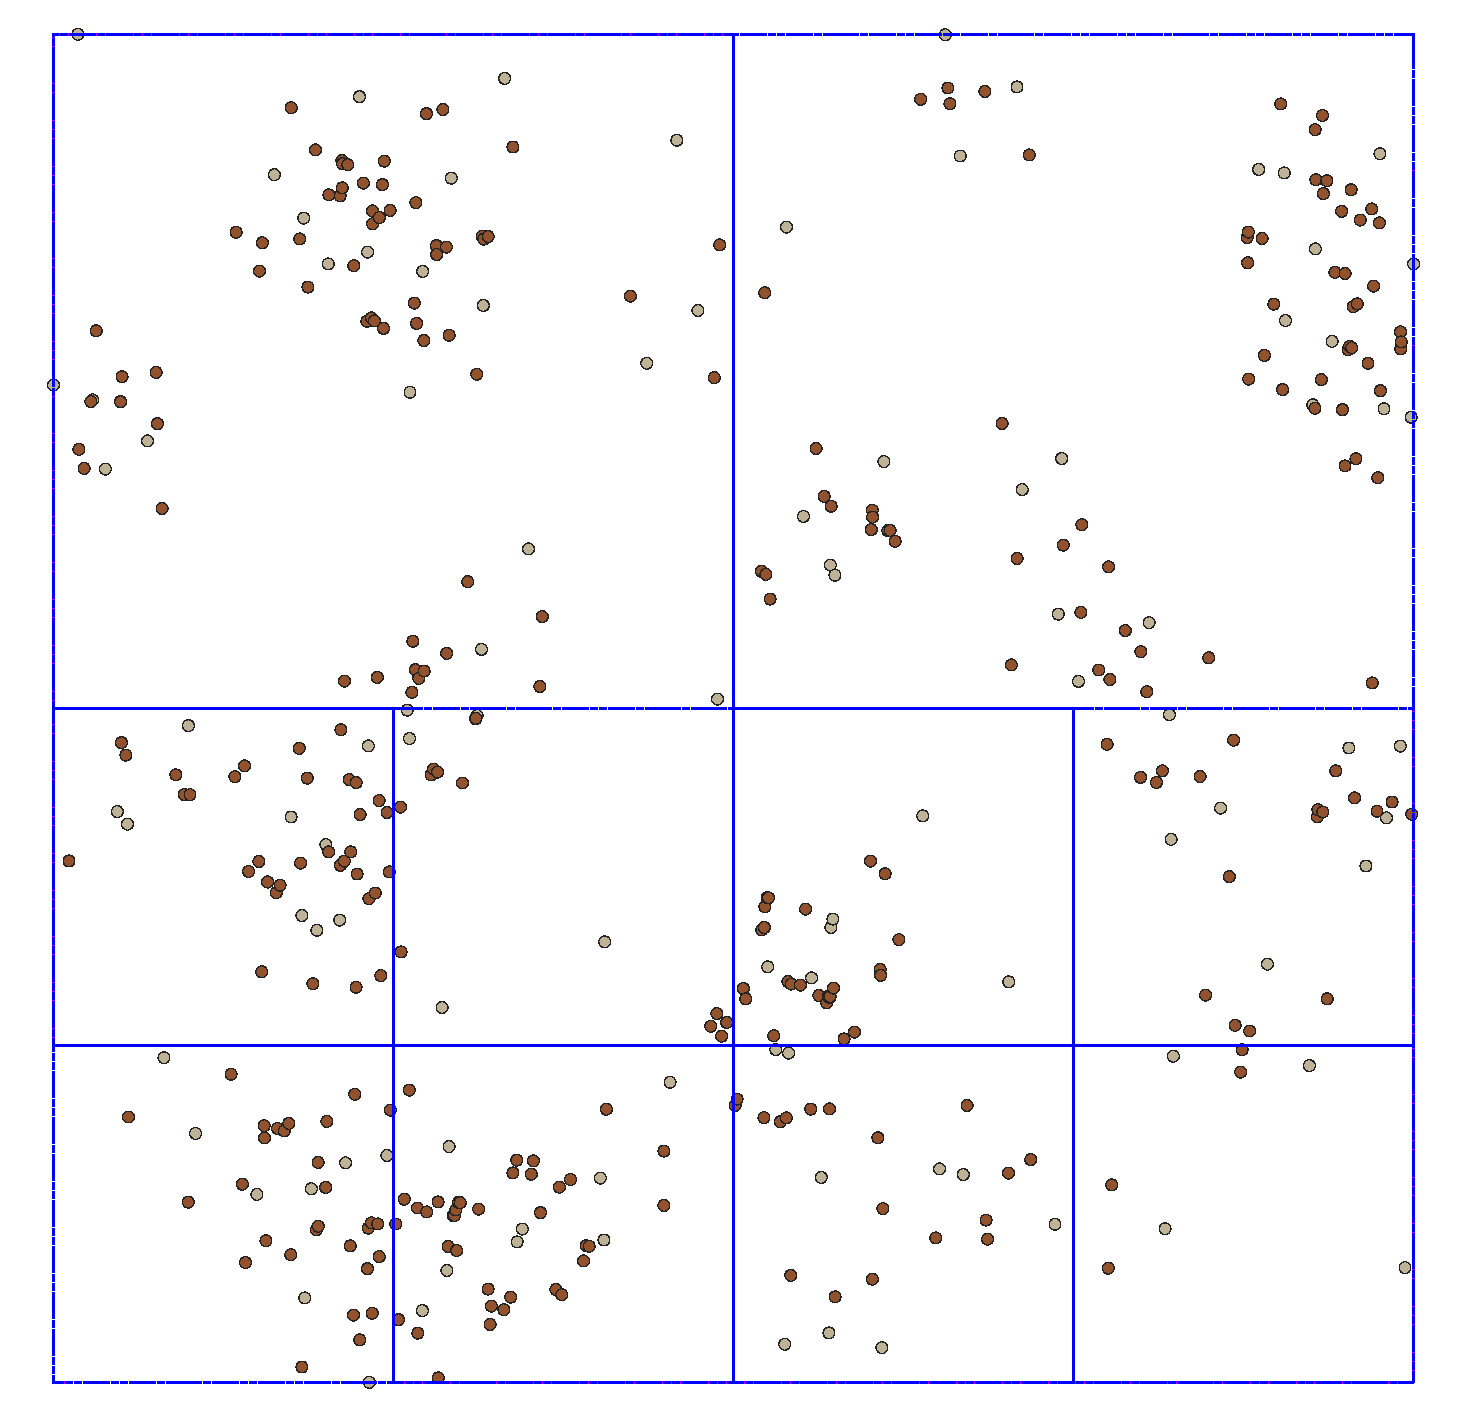
\includegraphics[width=0.65\textwidth]{figures/03-Centers}
\end{frame}

\begin{frame}{Global Parititons...}
    \centering
    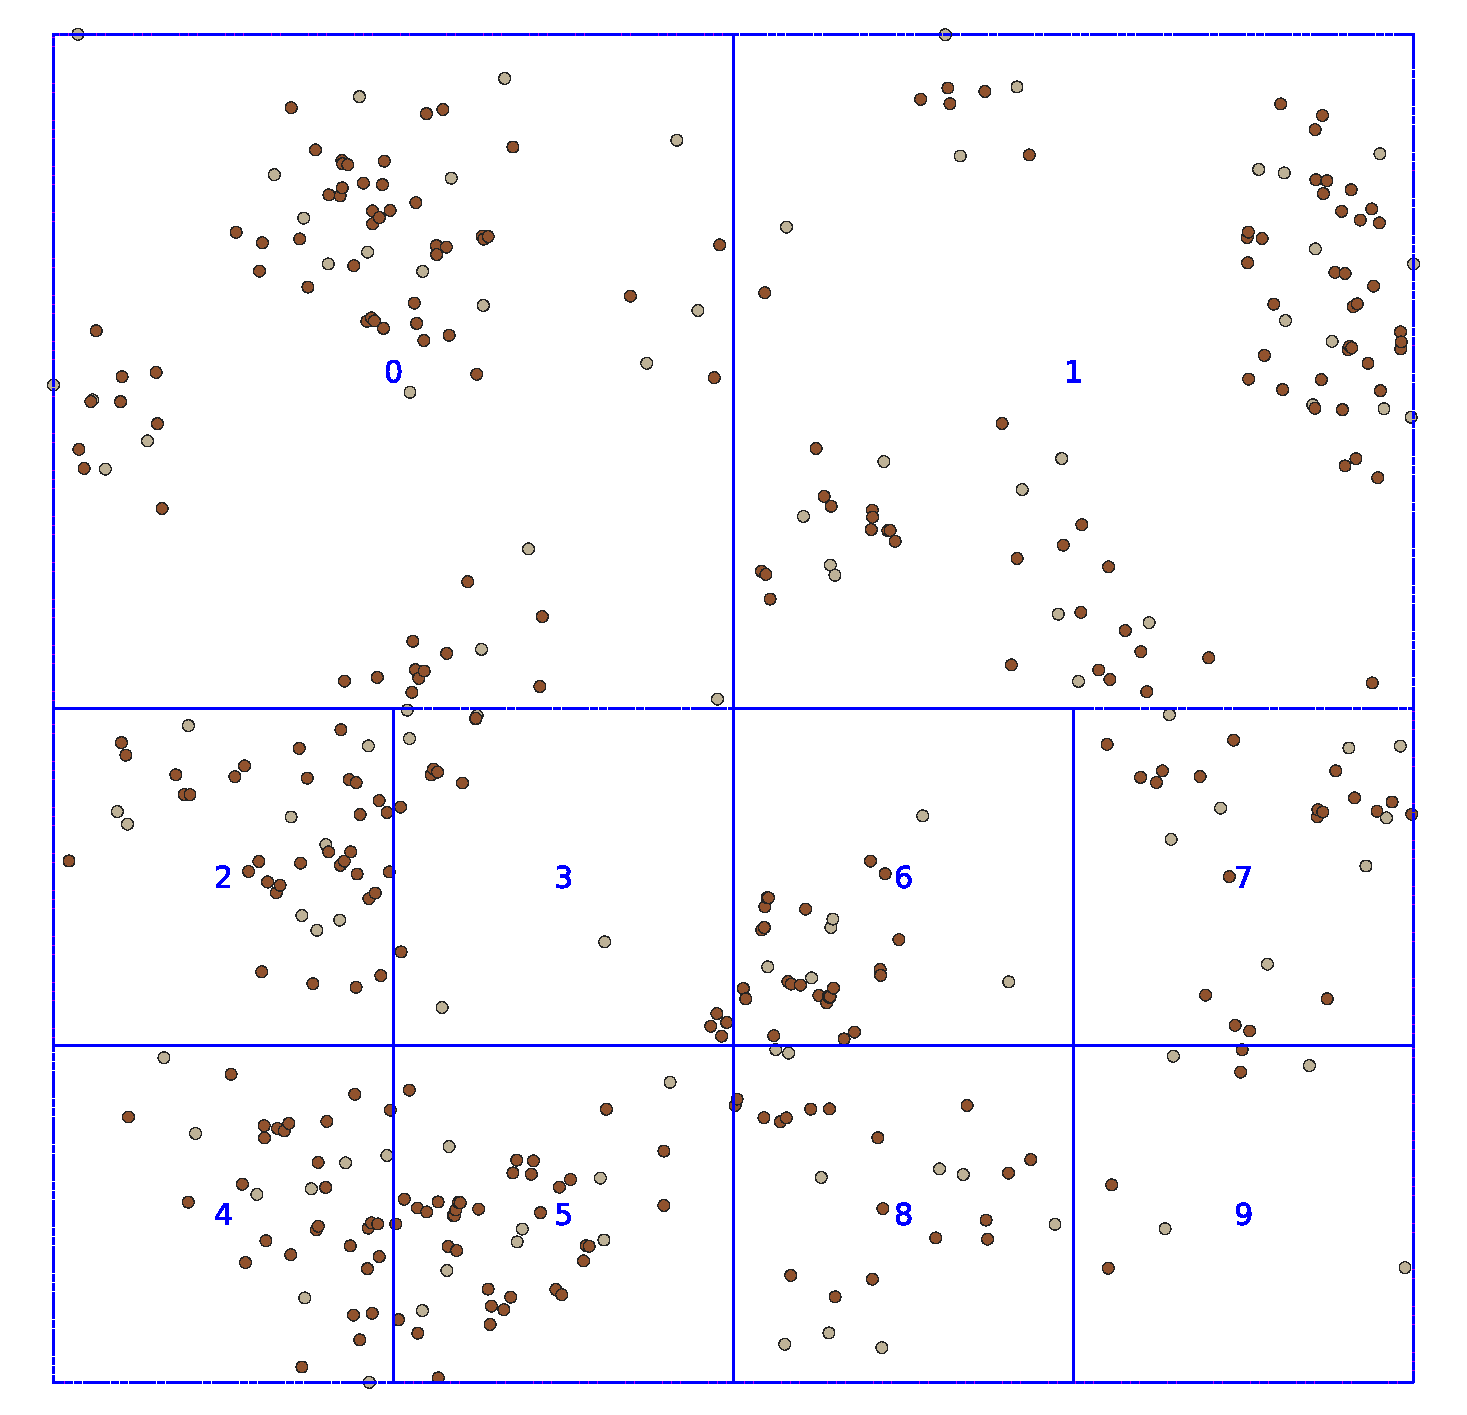
\includegraphics[width=0.65\textwidth]{figures/04-GPartitions}
\end{frame}

\begin{frame}{Local Quadtree...}
    Input: A sequence of Points (I have marked which ones are points and which ones are centers)
    \begin{enumerate}
     \item Take a sample from the sequence
     \item Build a quadtree with the sample
     \item Query the quadtree with the rest of the sequence to extract the corresponding leaf or leaves.
        \begin{enumerate}
            \item In case of a center, query its corresponding envelope.
        \end{enumerate}
     \item Match items in the same leaf and combine centers and points.
    \end{enumerate}
\end{frame}
\begin{frame}{Partition 0...}
    \centering
    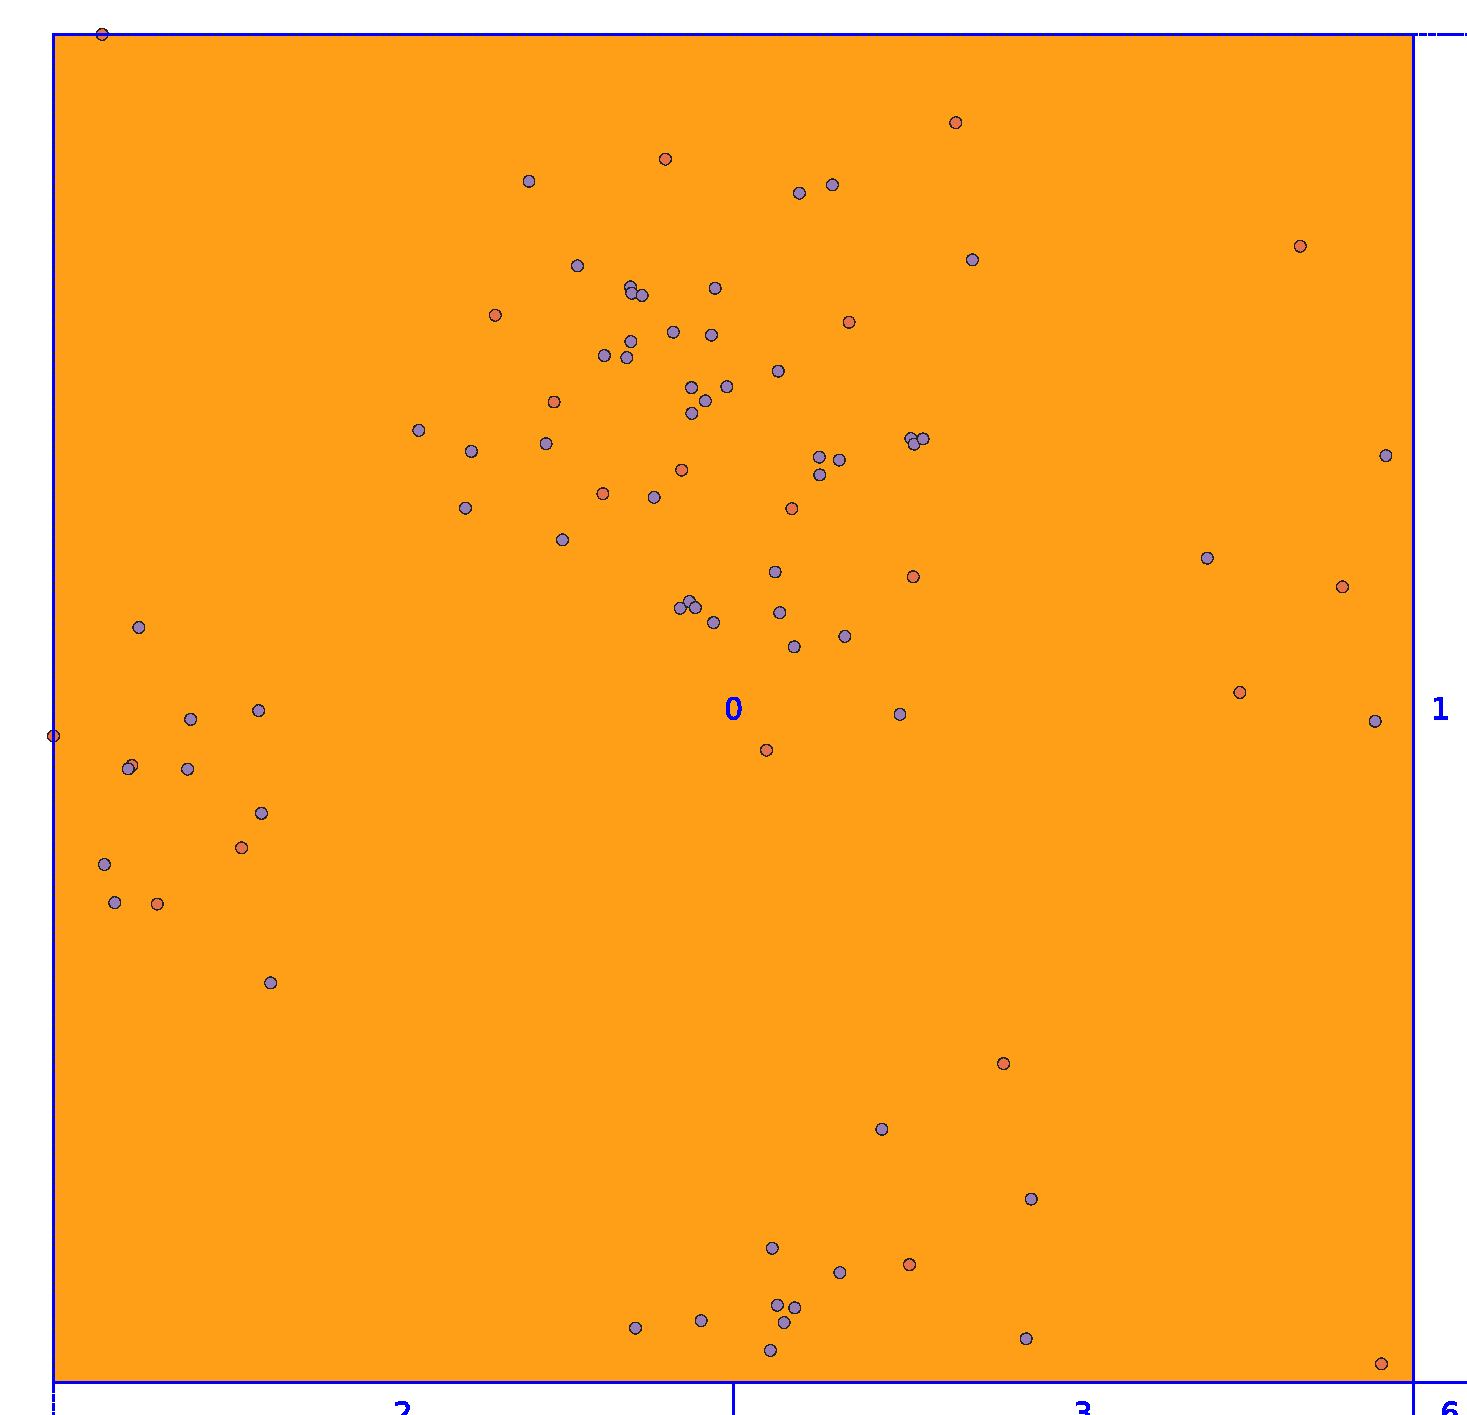
\includegraphics[width=0.65\textwidth]{figures/05-Partition0}
\end{frame}
\begin{frame}{Local Quadtree...}
    \centering
    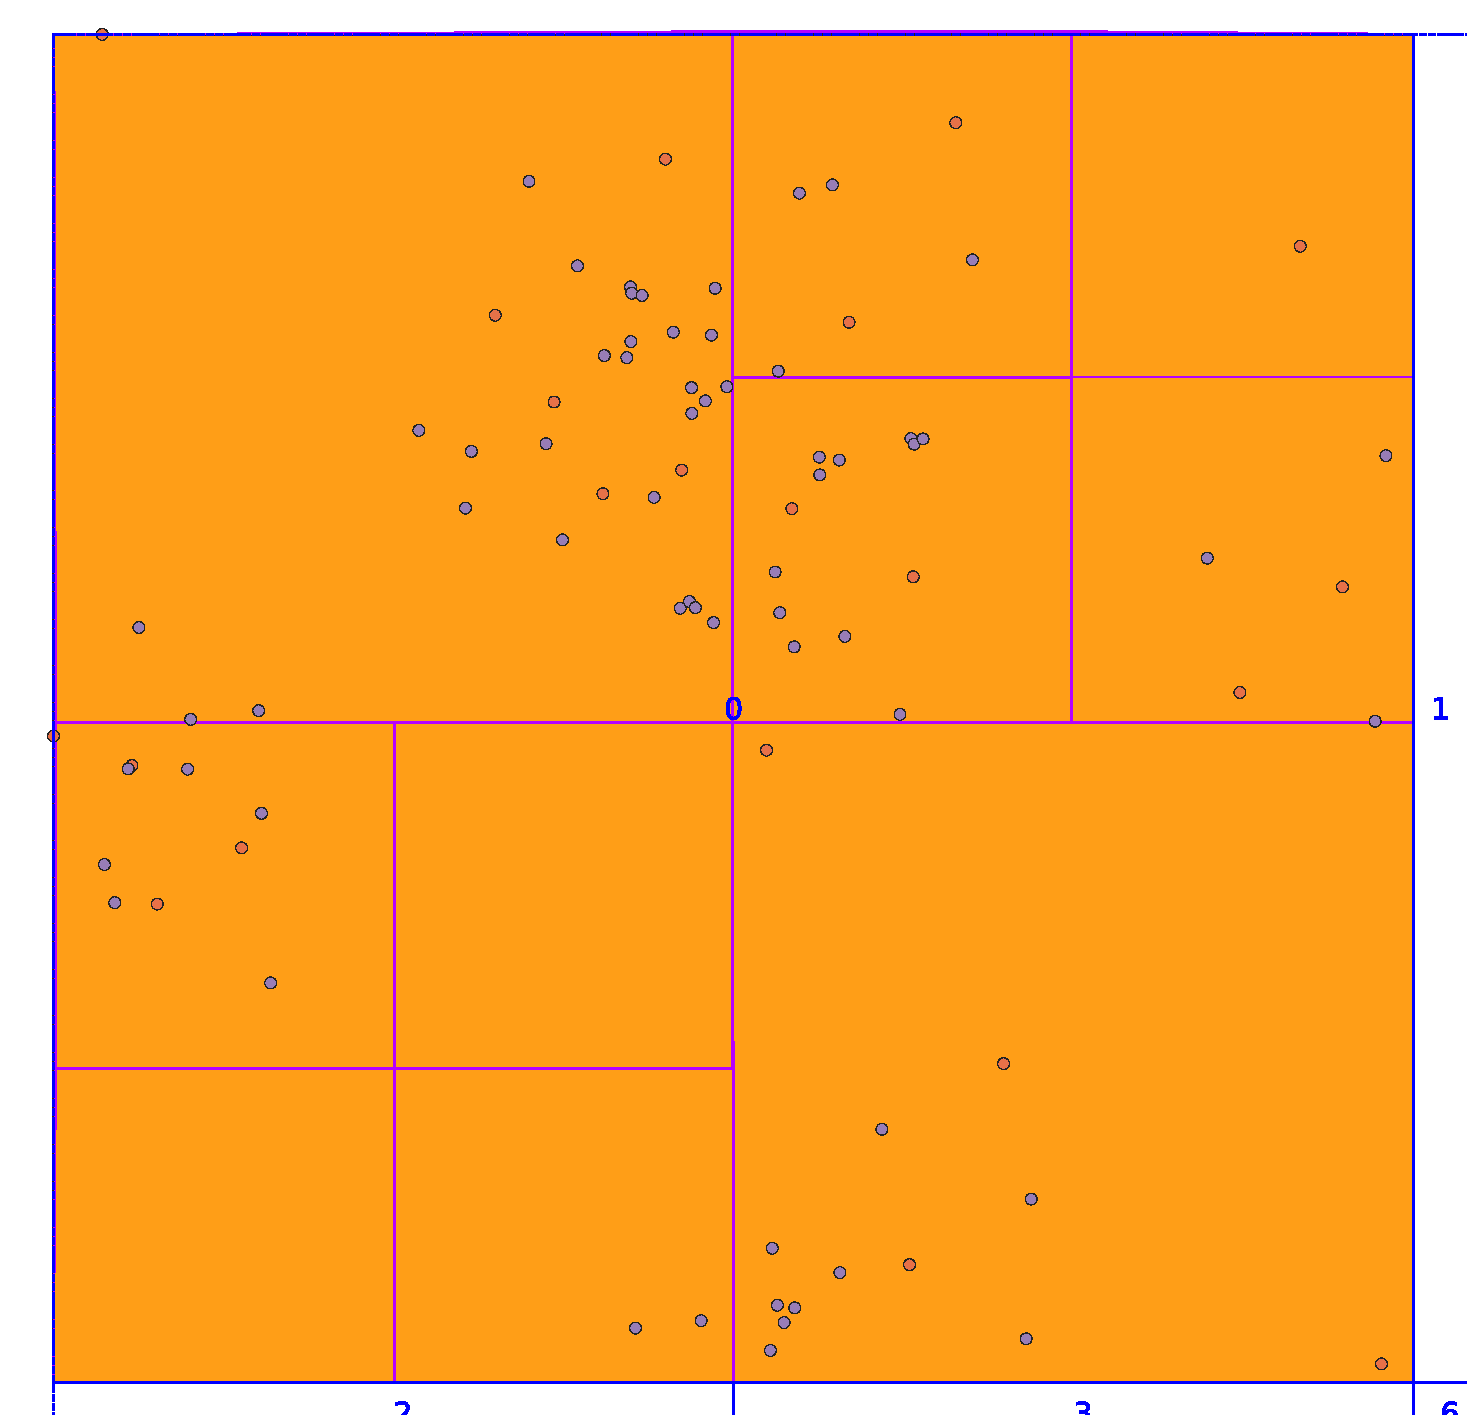
\includegraphics[width=0.65\textwidth]{figures/06-LQuadtree}
\end{frame}
\begin{frame}{What is the problem?}
    \begin{itemize}
        \item Construction of the quadtree takes most of the time.
        \item Difficult to tune good quadtrees.  Most of the time it generates very large quadtrees.
    \end{itemize}
\end{frame}

\begin{frame}{Local Grids...}
    Input: An index of Points (I can query the index to extract points and identify if it is a point or center)
    \begin{enumerate}
     \item Create a set of regular grids based on the extension of the Partition's boundary.
     \item For each grid:
        \begin{enumerate}
            \item query the index to retrieve the associated items.
            \item combine points and centers.
        \end{enumerate}
    \end{enumerate}
\end{frame}
\begin{frame}{Partition 0...}
    \centering
    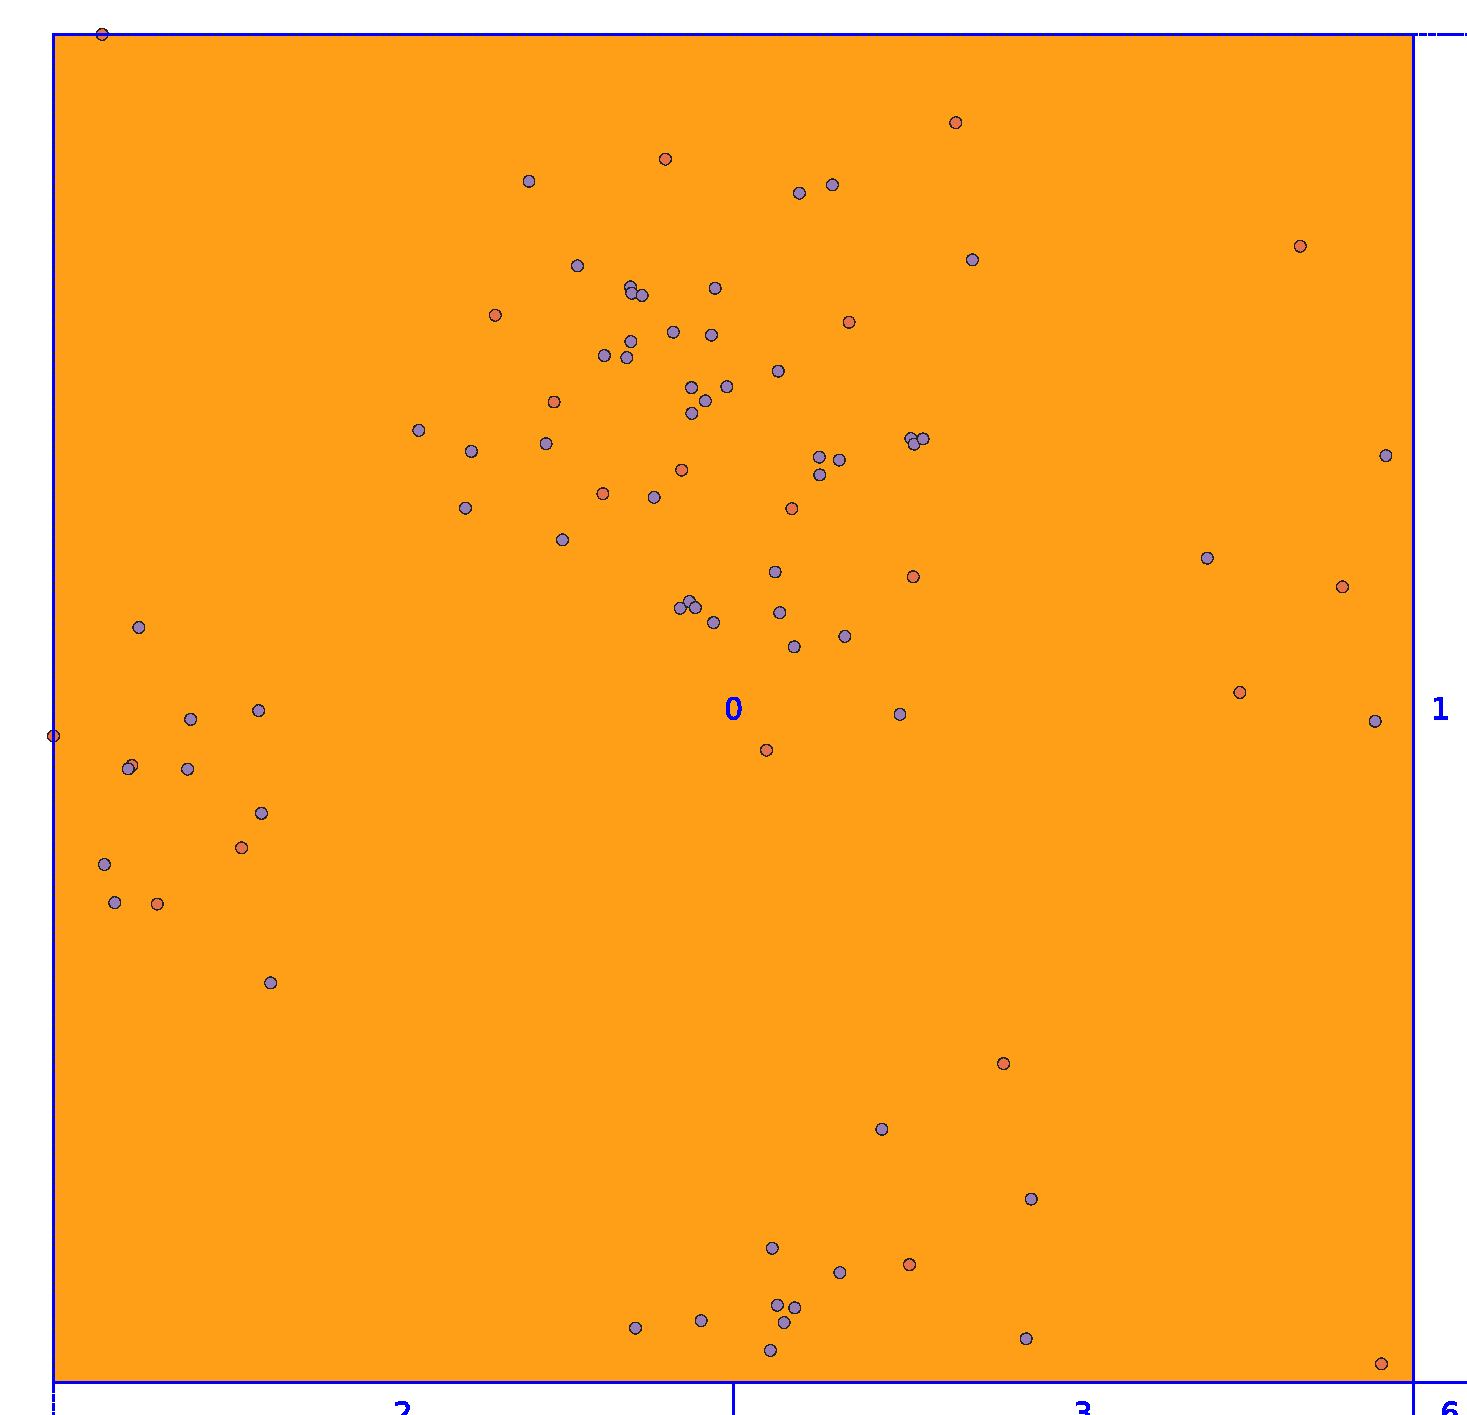
\includegraphics[width=0.65\textwidth]{figures/05-Partition0}
\end{frame}
\begin{frame}{Local Grid...}
    \centering
    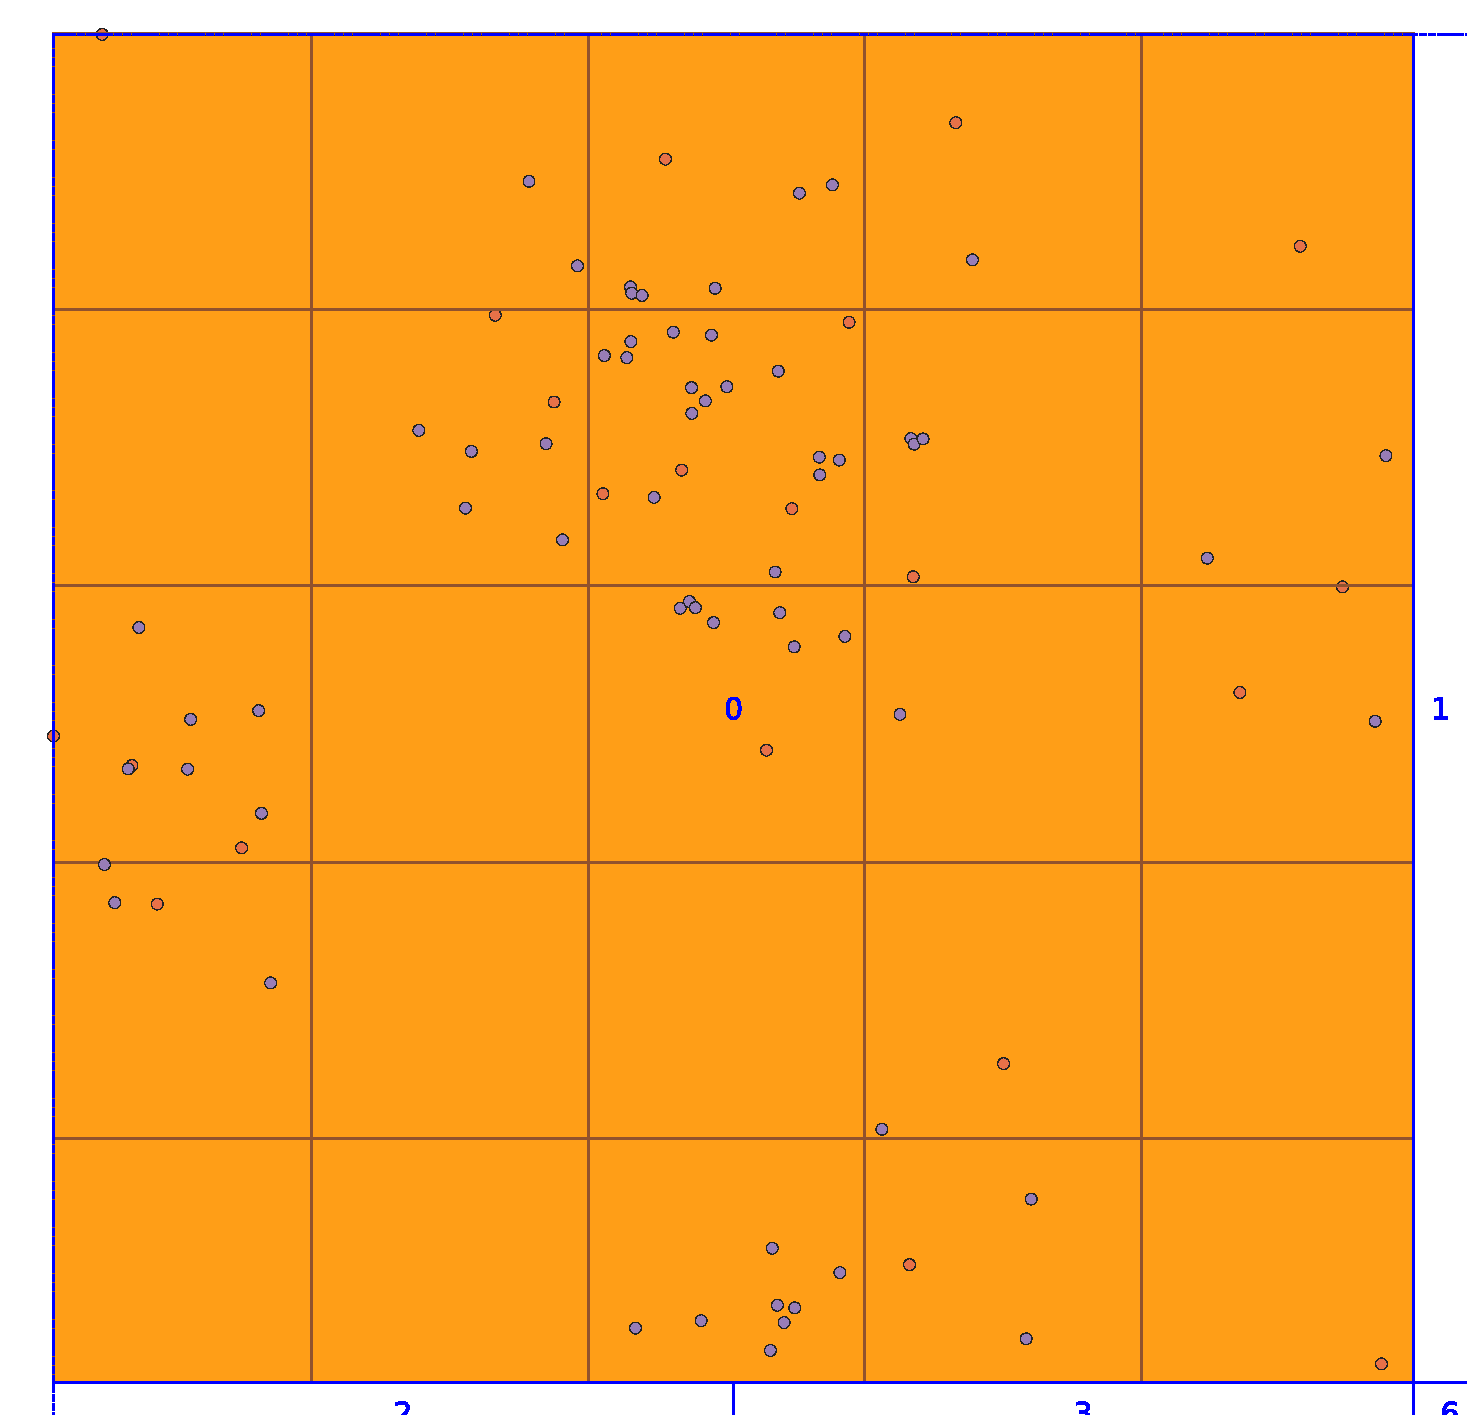
\includegraphics[width=0.65\textwidth]{figures/07-LGrids}
\end{frame}
\begin{frame}{What is the problem?}
    \begin{itemize}
        \item The JTS quadtree provided by GeoSpark as local index cannot retrieve leaves' MBRs.
        \item I can avoid the use of the local index but I have to solve the replication of centers manually.
    \end{itemize}
\end{frame}

\begin{frame}{What's next?}
    \begin{itemize}
        \item Double-check the local quadtree strategy.
        \item Work on local grids but avoid using an extra index.
        \item Explore other libraries: RTrees or KDBTrees.
    \end{itemize}
\end{frame}


\end{document}
